\subsection{Learning the Speediness in Videos}
\begin{frame}[allowframebreaks]{Learning the Speediness in Videos}
    \textbf{Learning Speediness} is a self-supervised learning approach that focuses on understanding the temporal dynamics of videos by learning to recognize or reconstruct videos at different playback speeds.

    \begin{itemize}
        \item \textbf{Speed Variation:} The model learns to predict or reconstruct video frames at various speeds, enhancing its understanding of temporal relationships.
        \item \textbf{Applications:} Useful for tasks like action recognition, video summarization, and temporal segmentation.
        \item \textbf{Goal:} To learn robust representations that capture the dynamics of video data across different temporal scales.
    \end{itemize}
\framebreak
    \textbf{Ultimate Goal:} Watch video content faster by adaptively speeding up the video
    \begin{figure}
        \centering
        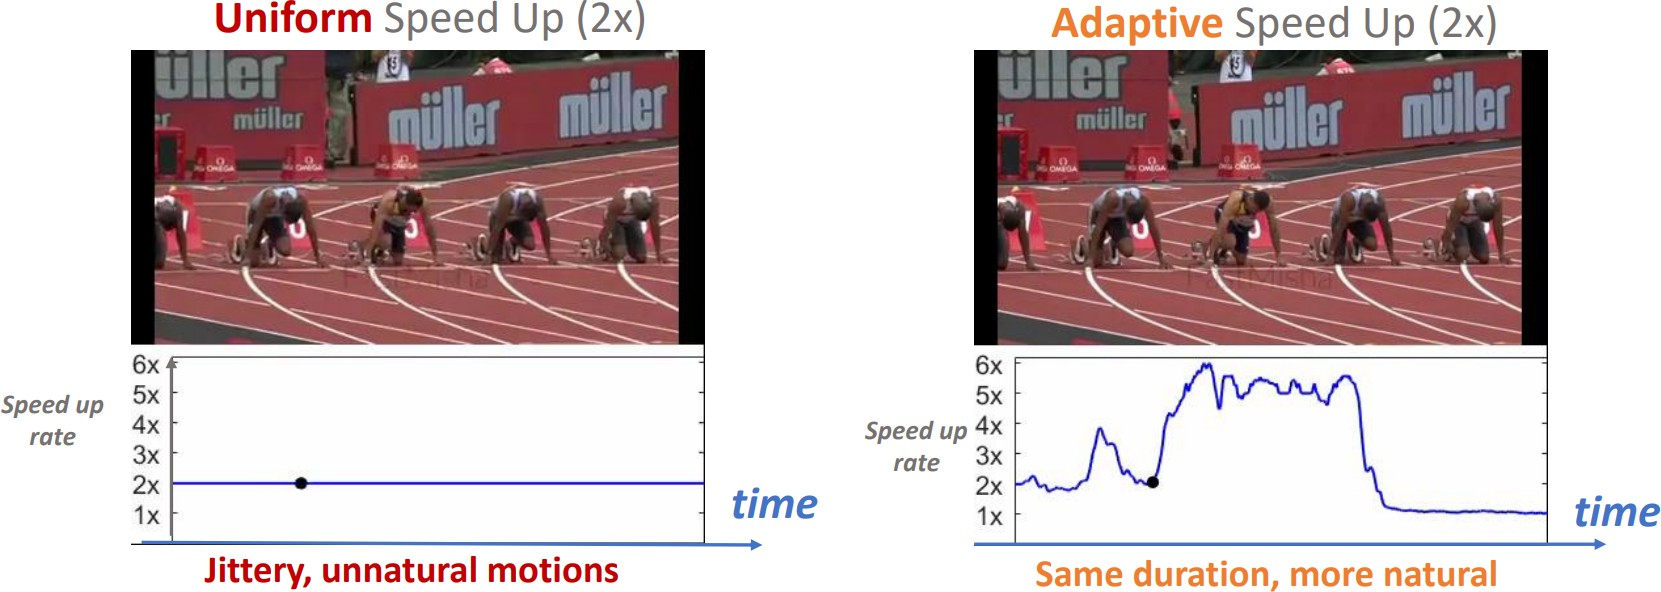
\includegraphics[width=1\textwidth,height=0.7\textheight,keepaspectratio]{images/video/slide_49_1_img.jpg}
    \end{figure}
    \footnotesize{[Joint work with: Sagie Benaim, Ariel Ephrat, Oran Lang, Inbar Mosseri, Bill Freeman, Miki Rubinstein and Michal Irani, CVPR 2020]}
\end{frame}